\chapter{Graph Connectivity}
\label{ch:graphcon::connect}

\begin{preamble}
This chapter presents a parallel graph connectivity algorithm that
uses graph contraction (more specifically star contraction). 
\end{preamble}

\begin{teachnote}
UPDATE THIS CHAPTER SO THAT THE EXAMPLES ARE MORE INTERESTING.  THEY SHOULD HAVE TWO CONNECTED COMPONENTS.
\end{teachnote}

\section{Preliminaries}
\label{sec:graphcon::connect::prelim}

\begin{definition}[The Graph Connectivity Problem]
\label{def:graphcon::connect::problem}
Given an undirected graph $G = (V,E)$, the \defn{graph-connectivity
  problem} requires finding all of the connected components of $G$ by
specifying the set of vertices in each component.
\end{definition}
%

\begin{flex}
\begin{assumption}[Graph Representation]
\label{graphcon::connect::graph-represent}
Throughout this chapter, we use an edge-set representation for graphs,
where every edge is represented as a pair of vertices, in both orders.
%
This is effectively equivalent to a directed graph representation of
undirected graphs with two arcs per edge.
%
As usual we use $n$ and $m$ to denote the number of vertices and edges respectively.
\end{assumption}

\begin{example}
\label{ex:graphcon::connect::graph-represent}

The edge-set representation of an undirected graph is shown below.

\begin{center}
  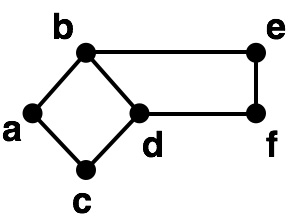
\includegraphics[width=2.0in]{./graph-contraction/media-connectivity/contract-example1.jpg}
\end{center}

\[
\begin{array}{lcl}
V & = & \cset{\vname{a},\vname{b},\vname{c},\vname{d},\vname{e},\vname{f}}\\
E & = &
\{(\vname{a},\vname{b}),(\vname{b},\vname{a}),(\vname{b},\vname{d}),(\vname{b},\vname{e}),(\vname{e},\vname{b}),(\vname{d},\vname{b}),(\vname{d},\vname{f}),(\vname{a},\vname{c}),
\\
& & ~~(\vname{c},\vname{a}),(\vname{c},\vname{d}),(\vname{d},\vname{c}),(\vname{d},\vname{f}),(\vname{f},\vname{d}),(\vname{e},\vname{f}),(\vname{f},\vname{e})\}
\end{array}
\]
\end{example}
\end{flex}
%% \begin{teachask}
%%   Solve the graph-connectivity problem by using one of the
%%   techniques recently covered earlier in the course.
%% \end{teachask}
%% %

\section{Algorithms for Connectivity}
\label{sec:graphcon::connect::alg}

\begin{gram}[Sequential Algorithms for Connectivity]
\label{gr:graphcon::connect::sequential}
The graph connectivity problem can be solved by using graph search as
follows. 
\begin{itemize}
\item Start at any vertex and find, using DFS or BFS, all vertices
  reachable from that vertex and mark them visited. This creates the
  first connected component.

\item 
Select another vertex, and if it has not already been visited, then
search from that vertex to create the second component. 
%
Repeat until all the vertices are considered.
%
%
\end{itemize}

This approach leads to perfectly sensible sequential algorithms for
graph connectivity, but the resulting algorithms have large span and are therefore poor parallel algorithms.
%

DFS is a purely sequential algorithm and has span $\Omega(m)$.
%
BFS can yield some parallelism but still the span of BFS is lower bounded by the diameter of a component, which can be as large as~$n-1$, e.g.,
a ``chain'' of $n$ vertices has diameter $n-1$.
%
Even when the diameter of the graph is small, the span can be high,
because we have to iterate over the components sequentially.
%
The span can is lower bounded by the number of components, which can be large.
\end{gram}


\begin{flex}
\begin{algorithm}[Component Count]
\label{alg:graphcon::connect::cc}

The pseudo-code below shows a graph-contraction based algorithm for
determining the number of connected components in a graph.
%
The call to $\cdvar{starPartition}$ (\algref{graphcon::star-partition}) on
Line~\linegcconnectccpartition{} returns the set of (centers)
super-vertices $V'$ and a table $P$ mapping every $v \in V$ to a $v'
\in V'$.
%


%
The set $V'$ defines the super-vertices of the quotient graph.
%
Line~\linegcconnectccedges{} completes the computation of the quotient
graph.
%
\begin{itemize}
\item It computes the edges of the quotient graph by 
routing the end points of each edge to the corresponding
super-vertices in $V'$, which is specified by the table $P$;
%
\item It  removes all self edges via the  filter $\cget{P}{u}
\neq \cget{P}{v}$.
%
\end{itemize}
%
The algorithm then recursively computes the number of connected components in the quotient graph.
%
Recursion bottoms out when the graph contains no edges, where the number of components is equal to the number of vertices.
%

\[
\begin{array}{ll}
1 & \cdvar{countComponents}~(G = (V,E)) =
\\ 
2 & ~~~~\cd{if}~|E| = 0~\cd{then}
\\
3 & ~~~~~~~~|V|
\\
4 & ~~~~\cd{else}
\\ 
5 & ~~~~~~~~\cd{let}
\\ 
6 & ~~~~~~~~~~~~(V',P) = \cdvar{starPartition}~(V,E)
\\
7 & ~~~~~~~~~~~~E' = \csetf{(\cget{P}{u},\cget{P}{v}) : (u,v) \in  E}{\cget{P}{u} \neq \cget{P}{v}} %
\\
8 & ~~~~~~~~~~~~R = \cdvar{countComponents}~(V',E')
\\
9 & ~~~~~~~~\cd{in}
\\
10 & ~~~~~~~~~~~~R
\\
11 & ~~~~~~~~\cd{end}
\end{array}
\]

%% \[
%% \begin{lstlisting}
%% countComponents $(G = (V,E))$ = 
%%   if $|E| = 0$ then $
%%     |V|$
%%   else 
%%     let 
%%       $(V',P)$ = starPartition $(V,E)$ @\label{line:graphcon::cc::partition}@
%%       $E'$ = $\csetf{(\cget{P}{u},\cget{P}{v}) : (u,v) \in E}{\cget{P}{u} \neq \cget{P}{v}}$ @\label{line:graphcon::cc::edges}@
%%     in
%%       countComponents $(V',E')$
%%     end
%% \end{lstlisting}

\end{algorithm}

\begin{example}
\label{ex:graphcon::connect::cc}

Consider an execution of $\cdvar{countComponents}$ that contracts the graph as follows.

\begin{center}
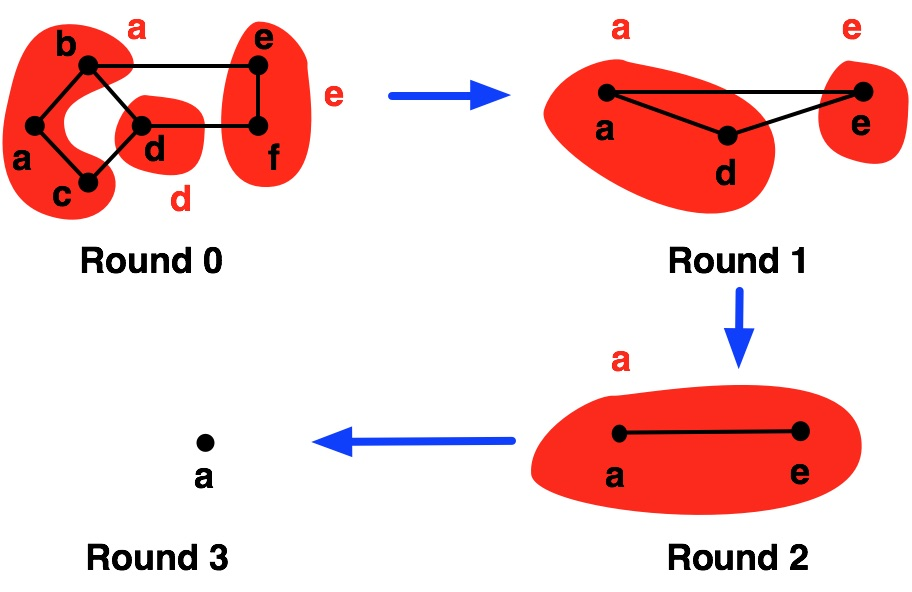
\includegraphics[width=4in]{./graph-contraction/media-connectivity/graph-contraction-example-1.jpg}
\end{center}
  
The values of $V'$, $P$, and $E'$ after each round of the 
contraction is shown below.
\[
\begin{array}{crcl}
  & V' & = & \cset{\vname{a},\vname{d},\vname{e}}\\
\mbox{Round } 1 & P' & = & 
 \cset{\vname{a} \mapsto \vname{a}, 
       \vname{b} \mapsto \vname{a}, 
       \vname{c} \mapsto \vname{a}, 
       \vname{d} \mapsto \vname{d}, 
       \vname{e} \mapsto \vname{e}, 
       \vname{f} \mapsto \vname{e}}\\
  & E' & = & \cset{(\vname{a},\vname{e}),
               (\vname{e},\vname{a}),
               (\vname{a},\vname{d}),
               (\vname{d},\vname{a}),
               (\vname{d},\vname{e}),
               (\vname{e},\vname{d})}\\[.1in]
  & V' & = & \cset{\vname{a},\vname{e}}\\
\mbox{Round } 2 & P' & = & 
 \cset{\vname{a} \mapsto \vname{a}, 
       \vname{d} \mapsto \vname{a}, 
       \vname{e} \mapsto \vname{e}}\\
  & E' & = & \cset{(\vname{a},\vname{e}),
               (\vname{e},\vname{a})}\\[.1in]
  & V' & = & \cset{\vname{a}}\\
\mbox{Round } 3 & P' & = & 
 \cset{\vname{a} \mapsto \vname{a}, 
       \vname{e} \mapsto \vname{a}}\\
  & E' & = & \cset{}
\end{array}
\]
\end{example}

\end{flex}

\begin{exercise}
Express $\cd{countComponents}$ in terms of higher order function
$\cd{starContract}$ (\algref{graphcon::star-contraction}) by
specifying the functions $\cd{base}$ and $\cd{expand}$.
\end{exercise}

\begin{gram}[Computing Components]
\label{graphcon::connect::cc-compontents}

%
We can modify 
\href{alg:graphcon::connect::cc}{algorithm for counting components} to compute the components themselves.
%
The idea is to construct recursively a mapping from vertices to their
components. 
%
The 
%
\href{alg:graphcon::connect::nc}{algorithm below} implements this idea.
\end{gram}

\begin{flex}

\begin{algorithm}[Graph Connectivity]
\label{alg:graphcon::connect::nc}

The algorithm below computes the connected components of the input
graph $G$ and returns a tuple consisting of
%
1) a representative for each component, and
2) a mapping from the vertices in the graph to the representative of their component. 
  
\[
\begin{array}{ll}
1 & \cdvar{connectedComponents}~(G = (V,E)) = 
\\
2 & ~~~~\cd{if}~|E| = 0~\cd{then}
\\ 
3 & ~~~~~~~~(V, \cset{v \mapsto v : v \in V})
\\
4 & ~~~~\cd{else}
\\ 
5 & ~~~~~~~~\cd{let}
\\
6 & ~~~~~~~~~~~~(V',P) = \cdvar{starPartition}~(V,E)
\\
7 & ~~~~~~~~~~~~E' = \csetf{(\cget{P}{u},\cget{P}{v}) : (u,v) \in E}{\cget{P}{u} \neq \cget{P}{v}}
\\
8 & ~~~~~~~~~~~~(V'',C) = \cdvar{connectedComponents}~(V',E')
\\
9 & ~~~~~~~~\cd{in}
\\
10 & ~~~~~~~~~~~~(V'', \cset{u \mapsto C[v] : (u \mapsto v) \in P}) % @\label{line:graphcon::nc::back}@
\\
11 & ~~~~~~~~\cd{end}
\end{array}
\]
% old code : \cset{v \mapsto \cget{P'}{\cget{P}{v}} : v \in V}
\end{algorithm}


\begin{example}
\label{ex:graphcon::connect::nc::1}

Applying $\cd{connectedComponents}$ to the following graph

\begin{center}
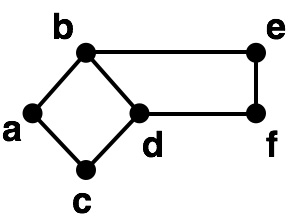
\includegraphics[width=2.0in]{./graph-contraction/media-connectivity/contract-example1.jpg}
\end{center}

might return:

\begin{eqnarray*}
(\cset{\vname{a}}, ~\cset{\vname{a} \mapsto \vname{a}, 
                          \vname{b} \mapsto \vname{a}, 
                          \vname{c} \mapsto \vname{a}, 
                          \vname{d} \mapsto \vname{a}, 
                          \vname{e} \mapsto \vname{a}, 
                          \vname{f} \mapsto \vname{a}})
\end{eqnarray*}

This is because there is a single component and all vertices will map
to that component label.  In this case $\vname{a}$ was picked as the
representative, but any of the initial vertices is a valid
representative, in which case all vertices would map to it.
\end{example}

\begin{example}
\label{ex:graphcon::connect::nc::2}

Consider the following graph.

\begin{center}
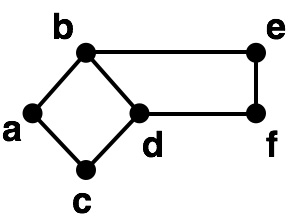
\includegraphics[width=2.0in]{./graph-contraction/media-connectivity/contract-example1.jpg}
\end{center}

Suppose that $\cd{starPartition}$ returns:
\[
\begin{array}{lcl}
V' & = & \cset{\vname{a},\vname{d},\vname{e}}\\
P & = & 
 \cset{\vname{a} \mapsto \vname{a}, \vname{b} \mapsto \vname{a}, 
       \vname{c} \mapsto \vname{a}, \vname{d} \mapsto \vname{d}, 
       \vname{e} \mapsto \vname{e}, \vname{f} \mapsto \vname{e}}.
\end{array}
\]
%
This pairing corresponds to the case where $a$, $d$ and $e$ are chosen
an centers.
%

Because the graph is connected, the recursive call to
$\cd{connectedComponents}~(V',E')$ will map all vertices in $V'$ to
the same vertex.  Lets say this vertex is $\vname{a}$ giving:
\[
\begin{array}{lcl}
V'' & = & \cset{\vname{a}}\\
P' & = & \cset{\vname{a} \mapsto \vname{a}, \vname{d} \mapsto \vname{a}, \vname{e} \mapsto \vname{a}}~.
\end{array}
\]
%
Now $\cset{u \mapsto P'[v] : (u \mapsto v) \in P}$ will for each
vertex-super-vertex pair in $P$, look up what that super-vertex got
mapped to in the recursive call.  For example, vertex $\vname{f}$ maps
to vertex $\vname{e}$ in $P$ so we look up $\vname{e}$ in $P'$, which
gives us $\vname{a}$ so we know that $\vname{f}$ is in the component
$\vname{a}.$  Overall the result is:
%
\[\cset{\vname{a} \mapsto \vname{a}, 
                          \vname{b} \mapsto \vname{a}, 
                          \vname{c} \mapsto \vname{a}, 
                          \vname{d} \mapsto \vname{a}, 
                          \vname{e} \mapsto \vname{a}, 
                          \vname{f} \mapsto \vname{a}}\;.\]
\end{example}
\end{flex}

\begin{note}
The only differences between the 
%
\href{alg:graphcon::connect::cc}{algorithm for counting components}
%
and the
%
\href{alg:graphcon::connect::nc}{algorithm for computing the components}
%
is the base case, and ``expansion step'' 
(Definition~\ref{def:graphcon::intro::graphcon::technique})
%
on Line~\linegcncback{} of Algorithm~\ref{alg:graphcon::connect::nc}.
%

In the base case instead of returning the size of $V$
returns all vertices in $V$ along with a mapping from each one to
itself.  This is a valid answer since if there are no edges each
vertex is its own component.  
%
In the inductive case, before returning
from the recursion, Line~\linegcncback{} updates the mapping $P$ from
vertices to super-vertices by looking up the component that the
super-vertex belongs to, which is given by $C$. 
%
This involves looking up $C[u]$ for every $(u \mapsto v) \in P$.  
%
If we view a mapping as a function, then the expansion step is equivalent to function composition, i.e., $C \circ P$.
\end{note}

\begin{exercise}
Express $\cd{countComponents}$ in terms of higher order function
$\cd{starContract}$ (\algref{graphcon::star-contraction}) by
specifying the functions $\cd{base}$ and $\cd{expand}$.
\end{exercise}


\begin{exercise}
What is the work and span of the
%
\href{alg:graphcon::connect::cc}{algorithm for counting components}
?
%
Explain your choice of the representation for the graph. 
%
What happens if you choose a different representation?
\end{exercise}
%

\begin{exercise}
What is the work and span of the
%
\href{alg:graphcon::connect::nc}{algorithm for computing the components}
?
%
Explain your choice of the representation for the graph.
%
What happens if you choose a different representation?
\end{exercise}
